\subsection{Photon-Gluon Fusion}

\begin{figure}
  \centering
  \begin{fmfgraph*}(200,150)
    \fmfleft{proton,gamma}
    \fmfright{proton',quark1,quark2}
    \fmf{fermion,width=2.5}{proton,v1}
    \fmf{fermion}{v1,proton'}
    \fmf{gluon}{v1,v2}
    \fmfblob{.15w}{v1}
    \fmf{fermion}{v2,quark1}
    \fmf{fermion}{v2,v3,quark2}
    \fmf{photon}{gamma,v3}

    % wow, it really feels like I should not have to do all of this
    \fmffixedx{0.}{v2,v3}
    \fmffixedy{0.}{v2,quark1}
    \fmffixedy{0.}{v3,quark2}
    \fmffixedy{0.}{v1,proton'}
    \fmffreeze
    \fmfshift{(0,-0.2h)}{v3}
    \fmfshift{(0.09w,-0.2h)}{quark2}
    \fmfshift{0,0.15h}{v1,proton'}
    
    % finally, add lines for outgoing quarks in struck proton
    \fmfi{plain}{vpath (__v1, __proton') shifted (thick*(-0.5,3.5))}
    \fmfi{plain}{vpath (__v1, __proton') shifted (thick*(-0.5,-3.5))}
  \end{fmfgraph*}
  \caption{Feynman diagram of photon-gluon fusion process}
\end{figure}


What's the problem with NLO analysis of these measurements?

Latest result from COMPASS analysis seems to be $\Delta g(x)/g(x) = -0.49~\pm~0.27(stat)~\pm~0.11(syst)$ at a scale $\mu^2 \sim 13 (GeV/c)^2$ and at an average gluon momentum fraction $<x>~\sim 0.11$ \cite{Alekseev:2009ey}.

%% Direct \Delta G figure without preliminary results
% \begin{figure}
%   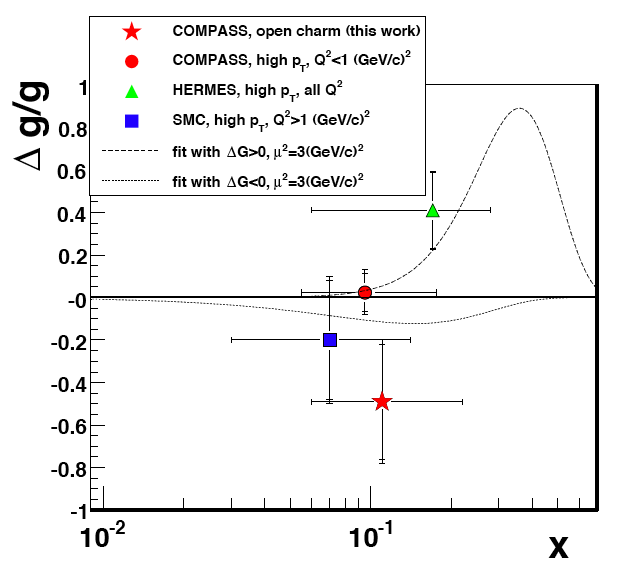
\includegraphics[width=1.0\textwidth]{figures/compass_deltag}
%   \caption{\cite{Alekseev:2009ey}}
% \end{figure}

\begin{figure}
  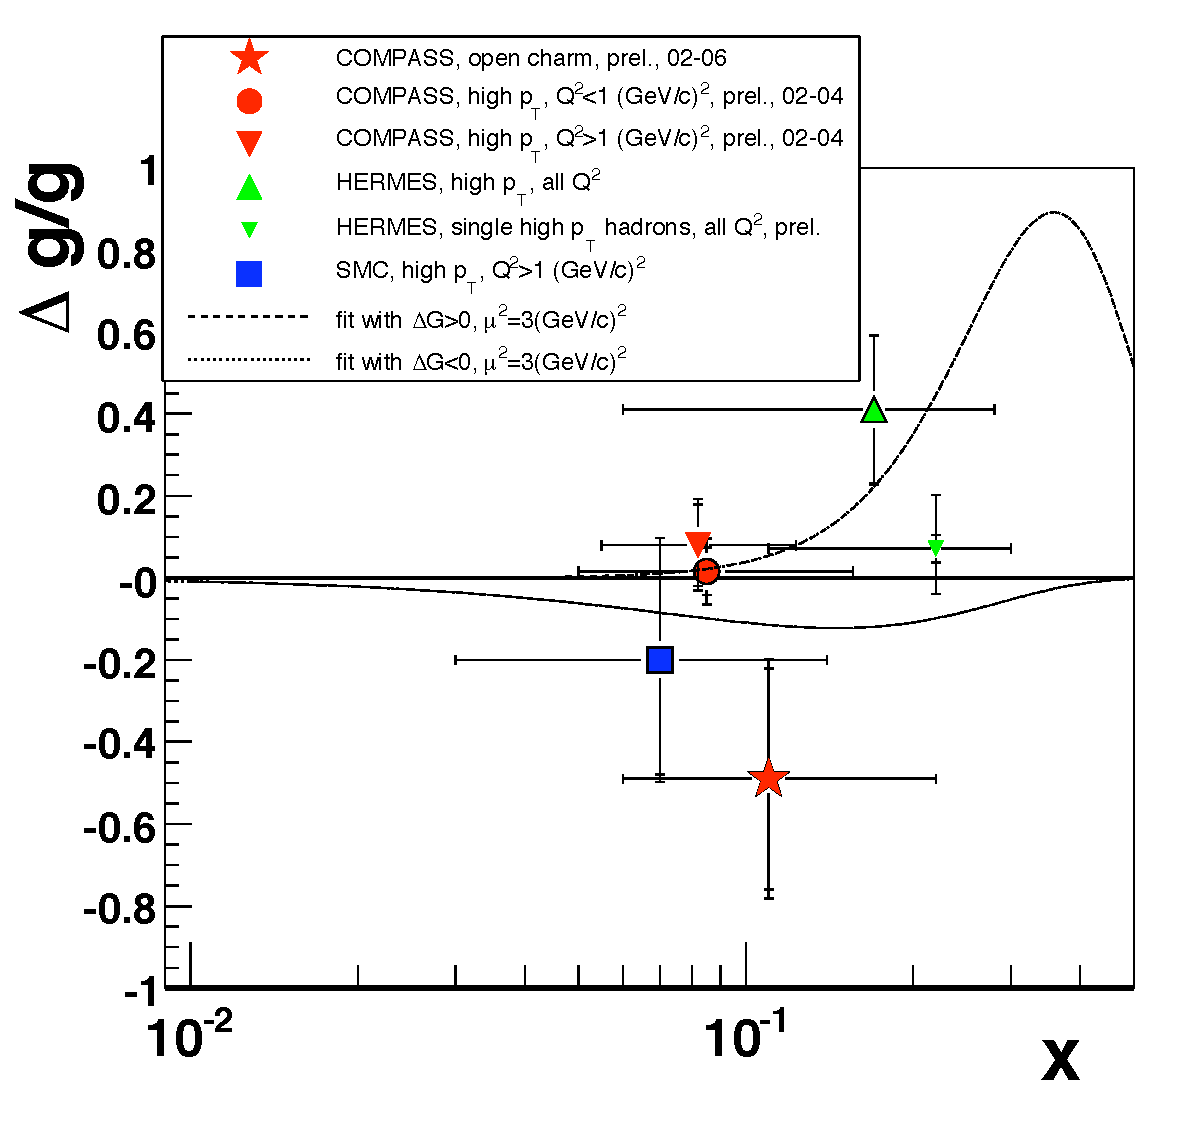
\includegraphics[width=1.0\textwidth]{figures/compass_deltag_with_prelim}
  \caption{this figure comes from DIS2008, but I don't see anything in SPIRES or the arXiv on it yet.  Kurek was the author}
\end{figure}